\documentclass[12pt, compress]{beamer} % ,t or ,b for top or bottom-aligned, compress for h-dots
\usepackage{graphicx}
\usepackage[absolute,overlay]{textpos} % to get full size picture
\usepackage{tikz}
\usepackage{csquotes}
\usepackage{hyperref}
\graphicspath{{images/}}

%%%%% BEAMER OPTIONS 

% NOTES PAGES
\usetheme{default}
\setbeameroption{show notes} % change to show to show notes
\setbeamertemplate{note page}[plain]
\addtobeamertemplate{note page}{\setlength{\parskip}{10pt}} % adds spaces to notes page

\setbeamertemplate{frametitle}[default][center] % centering titles
%\setbeamertemplate{footline} % footnote with sections
%{
%	\begin{beamercolorbox}[center]{section in head/foot}
%	\vskip12pt % distance from top 
%	\insertnavigation{\textwidth}
%	\vskip4pt % distance from bottom
%	\end{beamercolorbox}
%}

% \setbeamertemplate{footline}{% add footnotes
   % \raisebox{5pt}{\makebox[\paperwidth]{\hfill\makebox[20pt]{\color{gray}
         % \scriptsize\insertframenumber}}}\hspace*{5pt}}

\beamertemplatenavigationsymbolsempty % gets rid of navigation bar
% \setbeamertemplate{mini frames}{} % gets rid of navigation circles

\addtobeamertemplate{frametitle}{\vspace*{.6cm}}{\vspace*{0.2cm}} % slide title spacing

% \beamerdefaultoverlayspecification{<+->} % uncovers everything in a step-wise fashion

%%%%% SECTION TITLE SLIDES

\AtBeginSection[]{
  \begin{frame}
  \vfill
  \centering
  \begin{beamercolorbox}[center]{title}
  	\vskip14pt
    \usebeamerfont{title}\insertsectionhead\par%
  \end{beamercolorbox}
  \vfill
  \end{frame}
}

\AtBeginSubsection[]{
  \begin{frame}
  \vfill
  \centering
  \begin{beamercolorbox}[center]{title}
  	\vskip14pt
    \usebeamerfont{title}\insertsubsectionhead\par %
  \end{beamercolorbox}
  \vfill
  \end{frame}
}

%%%%% COLORS 

\definecolor{textcolor}{RGB}{24,24,24} % sets main text color
\definecolor{background}{RGB}{255,255,255} % sets background to white
%\definecolor{background}{RGB}{24,24,24} % sets background to black
%\definecolor{title}{RGB}{107,174,214}
%\definecolor{subtitle}{RGB}{102,255,204}
\definecolor{hilight}{RGB}{102,255,204}
\definecolor{vhilight}{RGB}{255,111,207}
\definecolor{medblue}{rgb}{.1,.35,1}
\definecolor{medgreen}{RGB}{22, 158, 58}
\definecolor{burntorange}{rgb}{0.8, 0.33, 0.0}
\definecolor{ceruleanblue}{rgb}{0.16, 0.32, 0.75}
\definecolor{darkblue}{RGB}{0,0,120}
\definecolor{gray}{RGB}{155,155,155}
\definecolor{lightgrey}{rgb}{.95,.95,.95}

\setbeamercolor{titlelike}{fg=ceruleanblue}
\setbeamercolor{subtitle}{fg=burntorange}
\setbeamercolor{framesubtitle}{fg=darkblue}
\setbeamercolor{institute}{fg=gray}
\setbeamercolor{normal text}{fg=textcolor, bg=background} % sets main background and font color
\setbeamercolor{item}{fg=burntorange}
\setbeamercolor{enumerate}{fg=burntorange}
\hypersetup{colorlinks, linkcolor=, urlcolor=burntorange} 
\let\oldtexttt\texttt% Store \texttt
\renewcommand{\texttt}[2][ceruleanblue]{\textcolor{#1}{\ttfamily #2}}% \texttt[<color>]{<stuff>}

%%%%% FONTS 
\usepackage[english]{babel}
\usefonttheme{professionalfonts}
\usefonttheme{serif}
\usepackage{fontspec}
\setmainfont[Ligatures=TeX]{Helvetica Light} % ligatures for em dash and quotation marks
\setbeamerfont{note page}{family*=pplx,size=\footnotesize} % Palatino for notes
\setbeamerfont{framesubtitle}{size=\small} 
\urlstyle{same} % make URLs in normal font, not mono-spaced


%%%%% SPACING
\let\noteitem\item % increase spacing between items
\renewcommand{\item}{ 
	\noteitem\vspace{\fill}
	}
\setlength{\tabcolsep}{0.5em} % horizontal padding for tables 

%%%%% MACROS
\newcommand{\bi}{\begin{itemize}}
\newcommand{\ei}{\end{itemize}}
\newcommand{\ig}{\includegraphics}
\newcommand{\subt}[1]{{\footnotesize \color{burntorange} {#1}}}
\newcommand{\nb}[1]{{\color{burntorange} {#1}}}

%%%%% TITLE MATERIAL %%%%

\title[Short Title]{Bringing the Scientific Process Into the Social Sciences}
\subtitle{A practical guide from start to finish \vspace{-20pt} }
\institute{\vspace{10pt} \ig[width = 40mm]{pdel.png}\vspace{10pt} \ig[width = 20mm]{UCSDlogo}}
\date[Short Occasion]{Craig McIntosh \& Julia Clark \\ Designing Field Experiments \\ 30 May 2017}

%%%%%%%%%%%%%%%%%%% BEGIN %%%%%%%%%%%%%%%%%%
\begin{document}


%%%%% TITLE PAGE

{\setbeamertemplate{footline}{} % no navigation
\frame{
  \titlepage
  \note{}
  }
}

%%%%%%%%%%%%%%%   	MOTIVATION	 %%%%%%%%%%%%%%%%
\section{Motivation}
\subsection{}
	\begin{frame}
		``\nb{Academia is a social enterprise} that is usually most successful when individual researchers \nb{compete and collaborate} in contributing toward common goals. 
		
		\bigskip
		In contrast, when we work in isolation on unrelated problems, ignoring work that has come before, we lose the benefits of evaluating each other's work, analyzing the same problem from different perspectives, improving measurement techniques and methods, and, most important, \nb{building on existing work rather than repeatedly reinventing the wheel}."
		
		\bigskip
		 -- Gary King 1995, p. 445
	\end{frame}

	\begin{frame}{(Social) Science!}
		 In order to \nb{accumulate knowledge}, we need to be able to replicate and extend the work that came before. This means we need to know:
		 
		 \begin{itemize}
		 	\item The universe of previous studies
		 	\item Their methods and specifications
		 	\item Their results (from ALL studies, not just the ones that got published!)
		 \end{itemize}
		 \bigskip
		 
		 $\rightarrow$ Requires research \nb{transparency}
	\end{frame}

	\begin{frame}{Without transparency, we have issues ...}
	
		\begin{itemize}
			\item \textbf{``Replication crisis"}--- studies fail to replicate (psych, econ, polisci, medicine, etc.)
			\item \textbf{Publication bias} --- published studies only represent fraction of results, biased toward significant positive findings
			\item \textbf{P-hacking/researcher degrees of freedom} --- published studies use only a fraction of possible specifications, biased toward significance 
			\item \textbf{Misconduct/fraud} --- easier to get away with!
		\end{itemize}			
		\bigskip
		
		$\rightarrow$ \nb{fragmented} and \nb{biased} body of knowledge
		
	\end{frame}
	
%%%%% REPLICATION CRISIS	
	
	\begin{frame}{``Replication Crisis"}
		\begin{itemize}
			\item \textbf{Problem:} In the past decade, many studies have failed to replicate across the social, behavioral, and medical sciences 
			\item \nb{\textbf{Ideally}}, replications help determine if original results are robust to alternative specifications or if they were due to \textit{random chance}.
			\item \nb{\textbf{In reality}}, failure to replicate often a result of ...
					\begin{itemize}
						\item Lack of transparency in sharing data/code
						\item Errors in data/code
						\item Misconduct or fraud 
					\end{itemize}
		\end{itemize}
	\end{frame}
		
	\begin{frame}{Dewald et al. (1986)}
	\centering
	Attempted to replicate 62 papers submitted to \textit{Journal of Money, Credit and Banking}, got data/code for only 22:
	
	\centering
	\bigskip
	\ig[width=.9\textwidth]{dewald.png}
		
	\end{frame}
	
	\begin{frame}{Fang et al. (2012}
		Review of 2,047 retracted biomedical and life-science articles on PubMed:
		
		\centering
		\bigskip
		\ig[width=.7\textwidth]{fang2012.png}
	\end{frame}
	
%	\begin{frame}{What is Replication?}
%	\centering
%	From \href{https://www.cgdev.org/sites/default/files/CGD-Working-Paper-399-Clemens-Meaning-Failed-Replications.pdf}{Clemens (2015)}:
%	
%	\bigskip
%		\ig[width=\textwidth]{clemens2015.png}
%	\end{frame}

%%%%% PUBLICATION BIAS

	\begin{frame}{Publication Bias}
		\begin{itemize}
			\item \textbf{``The File Drawer Problem":} Studies more likely to be published when findings are significant $\rightarrow$ studies with null (or negative) findings are hidden
			\item \textbf{Result:} Missing full universe of studies and results; what we believe to be a solid body of evidence could be due to random chance (e.g., if we expect 5\% of results of all studies to be significant)
		\end{itemize}		
	\end{frame}

	\begin{frame}{Publication Bias}
		\centering
		Increase in \% of papers with positive results over time, across scientific disciplines (Fanelli 2010, 2011):
		
		
		\bigskip
		\ig[width=\textwidth]{fanelli2011.png}
	\end{frame}
	
%		\begin{frame}{Publication Bias}
%		\centering
%	
%		\bigskip
%		\ig[width=\textwidth]{fanelli2010.png}
%	\end{frame}
	
	\begin{frame}{Bias in the Social Sciences}
		\centering
		Strong results 60pp more likely to be written up than null results, 40pp more likely to be published (Franco, Malhotra, Simonovits 2014):
		
		\bigskip
		\ig[width=\textwidth]{franco2014.png}
	\end{frame}

	\begin{frame}{This has consequences!}
		\centering
		E.g., studies that agree with FDA decisions more likely to be published (Turner et al. 2008):
		
		\bigskip
		\centering
		\ig[width=.5\textwidth]{turner2008a.png}	
	\end{frame}
	
%%%%% P-HACKING

	\begin{frame}{About P-Hacking (AKA fishing, data mining, specification searching, etc.)}
		\begin{itemize}
			\item \textbf{Motive:} Researchers have incentives (from journals, tenure requirements, etc.) to find significance
			\item \textbf{Opportunity:} Researchers also have many ``degrees of freedom" (RDF) in the design and analysis of a study $\rightarrow$ ``p-hacking" (may not always be intentional! see Gelman \& Loken 2013)
			\item \textbf{Result:} Biased evidence base (also contributes to replication crisis)
		\end{itemize}
	\end{frame}
	
	\begin{frame}{Evidence of P-Hacking}
		\centering
		Brodeur et al. (2016):
		
		\bigskip
		\ig[width=\textwidth]{brodeur2016.png}
	\end{frame}
	
	\begin{frame}{Researcher Degrees of Freedom}
		\href{https://osf.io/umq8d/}{Wicherts et al. 2016} identify 34 key RDFs (see article for full list):
		
		\bigskip
		\ig[width=\textwidth]{wicherts2016.png}
		...
	\end{frame}

%%%%% MISCONDUCT & FRAUD	

	\begin{frame}{Misconduct \& Fraud}
		\begin{itemize}
			\item \textbf{Includes}: Falsifying some or all data and/or results, as well as plagiarism and other forms of misconduct
			\item \textbf{Result:} False or biased evidence base,  (also contributes to replication crisis)
			\item \nb{\textbf{Note}:} Fabrication of data (e.g., \href{https://fivethirtyeight.com/features/how-two-grad-students-uncovered-michael-lacour-fraud-and-a-way-to-change-opinions-on-transgender-rights/}{LaCour}, \href{http://nautil.us/issue/24/error/how-the-biggest-fabricator-in-science-got-caught}{Fujii}, \href{http://andrewgelman.com/2014/06/24/linear-true-curious-case-jens-forster/}{Foster}, \href{https://www.theguardian.com/science/2017/feb/01/high-tech-war-on-science}{Staple}) less common than other ``questionable research practices"
		\end{itemize}
	\end{frame}
	
	\begin{frame}{Questionable Research Practices}
		 \centering
		 Survey of 2000 psychologists (John et al. 2012):
		 
		 \ig[width=.9\textwidth]{john2012.png}
	\end{frame}
		
%%%%% SOLUTIONS

%	\begin{frame}{Maximize your contribution to scientific knowledge}
%		 \textit{Not enough to have interesting results}. Make sure your research materials (code, data, etc.) are:
%		\begin{itemize}
%			\item \nb{Visible}---registered in universe, even if not published
% 			\item \nb{Available}---publicly shared 
%			\item \nb{Legible}---complete, readable by humans
%			\item \nb{Replicable}---reproduce results
%		\end{itemize}
%	\end{frame}
	
	\begin{frame}{Good news, everyone!}
		\nb{Norms are changing.} Smart people are working on these issues in the social sciences and developing standards and tools to help throughout the \nb{research lifecycle}. 
		
		\begin{itemize}
			\item PDEL, BITSS, OSF, DART, Dataverse, EGAP, etc. etc. 
		\end{itemize}
	\end{frame}

	\begin{frame}{Research Lifecycle}
		\ig[width=\textwidth]{lifecycle.png}
	\end{frame}

%	\note{Clear steps you can take at every stage of the research process [NOTE: Here, we're focusing on individual solutions. For more disciplinary solutions, see additional notes at the end]:
%		\begin{enumerate}
%			\noteitem Design---BEFORE data collection, register your study [addresses publication bias] and submit a pre-analysis plan [addresses researcher degrees of freedom]. Complying with IRB requirements is also a key element of ethical research that meets disciplinary standards, but we won't go into that here. 
%			\noteitem Analysis---During data analysis and write-up, use good data and file management practices [helps with transparency and reproducibility], and also make sure you're following your pre-analysis plan!
%			\noteitem Dissemination---Once the analysis is done, you should prepare files for replication and upload data and code in online repositories. This is increasingly required by journals.
%		\end{enumerate}
%		Once your results enter the universe, they can be used by others for replication and meta analysis --> one datapoint among many.  
%		}

%%%%%%%%%%%%%%%  	PHASE 1: DESIGN	 %%%%%%%%%%%%%%
\section{Phase I: Design}

	\begin{frame}{Steps}
	  	\centering
	  	\ig[width=\textwidth]{i_design}
	\end{frame}

%%%%% REGISTRATION	

\subsection{1. Registration}

	\begin{frame}{About Registration}
		\begin{itemize}
			\item \textbf{What:} Enter your study into the appropriate disciplinary ``registry"---basically a requirement for experiments (especially in medicine)
			\item \textbf{Why:} To combat the file-drawer problem, publication bias [\nb{visibility}]; also, stake out intellectual claim!
		\end{itemize}
	\end{frame}
	
%	\note{\bigskip
%		Registration is a partial, though not complete, solution to the file-drawer problem that results in publication bias. By registering your study in the appropriate repository, it is recorded as a datapoint in the universe of knowledge so that---even if not published in a journal---others can find and build off of it. 
%		
%		\bigskip
%		
%		This is now the norm in experimental work, particularly in medicine, where top journals (e.g., ICMJE) won't publish RCTs that haven't been registered. Less registration for observational work, where there is still an ongoing debate about its merits.}
	
	\begin{frame}{Where to Register}
		\begin{itemize}
			\item \textbf{American Economics Association (AEA):} \url{http://socialscienceregistry.org}
			\item \textbf{Experiments in Governance and Politics (EGAP):} \url{http://egap.org/design-registration}
			\item \textbf{Registry for International Development Impact Evaluations (3ie):} \url{http://ridie.3ieimpact.org}
			\item \textbf{Open Science Framework:} \url{http://osf.io}---OSF is integrated with other formats, soon with AEA!
			\item \url{http://aspredicted.org}
		\end{itemize}
		\end{frame}
	
	\begin{frame}{AEA}
		To register an experimental study with AEA ...
		
		\begin{enumerate}
			\item Create an account at \url{https://www.socialscienceregistry.org}
			\item Click on ``register a trial" and enter basic information---including title, country, status, keyword, abstract, start and end dates, outcomes, experimental design, whether treatment clustered, planned number of clusters and observations, IRB information
		\end{enumerate}
	\end{frame}	
		
	\begin{frame}{EGAP}
		To register an experimental (or non-experimental) study with EGAP ... 
		
		\begin{enumerate}
			\item If you're not already in the EGAP author database, go to \url{http://egap.org/node/add/people} to add your name and basic information 
			\item Go to \url{http://egap.org/node/add/registration} and complete the registration form---including faculty affiliation, prospective vs. retrospective, whether experimental, start date, background on study, hypotheses to be tested, basic research design, sample size, whether power analysis, IRB information, and keywords
		\end{enumerate}
	\end{frame}	

%%%%% PRE-ANALYSIS PLANS	
	
\subsection{2. Pre-Analysis Plan}

	\begin{frame}{About Pre-Analysis Plans (PAP)}
		\begin{itemize}
			\item \textbf{What:} Detailed description of research design and data analysis plans, submitted to a registry BEFORE looking at the data.
			\item \textbf{Why:} 
				\begin{itemize}
				 	\item Tie your hands for data analysis (address researcher degrees of freedom, multiple hypothesis testing, etc.)
				 	\item Distinguish between \textit{confirmatory} and \textit{exploratory} analysis
				 	\item Boost credibility of research (get a badge from OSF!)
				 	\item Transparent methods make it easier for others to build on your work
				\end{itemize}
		\end{itemize}
	\end{frame}
	
	\begin{frame}{PAP vs. Registration}
		Registration often---but not always---includes a pre-analysis plan. BUT, purpose is different ...
		
		\begin{itemize}
			\item \textbf{Registration addresses publication bias}---study enters the universe, no matter the outcome 
			\item \textbf{PAP adresses p-hacking}---separate confirmatory vs. exploratory analysis
		\end{itemize}	
		\bigskip
	\end{frame}

	\begin{frame}{Where to Submit a PAP}
		Generally, upload as \textit{part} of registration process ...
		
		\begin{itemize}
			\item \textbf{American Economics Association (AEA):} \url{http://socialscienceregistry.org} 
			\item \textbf{Experiments in Governance and Politics (EGAP):} \url{http://egap.org/design-registration}
			\item \textbf{Registry for International Development Impact Evaluations (3ie):} \url{http://ridie.3ieimpact.org}
			\item \textbf{Open Science Framework:} \url{http://osf.io}
		\end{itemize}
		\end{frame}	
		
	\begin{frame}{No universal standard, recommendations include ... }
		\footnotesize
		\begin{enumerate}
			\item \textbf{Background:} Abstract, motivation, questions
			\item \textbf{Design:} Treatment, sampling \& randomization, attrition, spillover, survey instruments, power calculations, plan for data collection, processing \& management
			\item \textbf{Analysis:} hypotheses (main, auxiliary), outcome measures (primary, secondary), variable operationalization, balance checks, estimation of treatment effects (ATE, ITT, TOT, etc.), HTEs (subgroups, interactions), covariates, standard errors, corrections for multiple hypothesis testing, missing values, outliers
			\item \textbf{Research team:} Members, affiliations, conflicts of interest
			\item \textbf{Logistics:} Fieldwork, timeline, budget
		\end{enumerate}
	\end{frame}	
	
	\begin{frame}{Tie your hands in the right places}
			\centering
			\ig[width = .8\textwidth]{pap_scale.png}
			
			\bigskip
			 $\rightarrow$ \textbf{PAP requires a lot of thought!} 
	\end{frame}
	
	\begin{frame}{Olken's PAP Checklist (2013)}
		\ig[width = \textwidth]{olken2013.png}
	\end{frame}

	\begin{frame}{Ongoing Debate}
		\begin{itemize}
			\item \href{https://www.aeaweb.org/articles?id=10.1257/jep.29.3.61}{Olken (2013)} on ``Promises and Perils of Pre-analysis Plans"
			\item \href{https://www.aeaweb.org/articles?id=10.1257/jep.29.3.81}{Coffman \& Niederle (2015)} argue that ``Pre-analysis Plans Have Limited Upside, Especially Where Replications Are Feasible"
			\item More debate on utility for observational work but can be done (see \href{http://onlinelibrary.wiley.com/doi/10.1111/0019-8676.00199/full}{Neumark 2001})
		\end{itemize}
	\end{frame}

%%%%% OSF	

	\begin{frame}{\textbf{Spotlight on OSF} \\ ``A scholarly commons to connect the entire research cycle"}
		(Trying to be) a one-stop hub for managing projects, collaboration, materials, with integrated registration, pre-analysis plans, file management (Dropbox), version control (GitHub), etc., across scientific disciplines. 	
			
		\bigskip
		... Make an account and explore at \url{https://osf.io/}
	\end{frame}
%
%	\begin{frame}
%		Click ``sign up" and enter your info ... \bigskip
%		
%		\ig[width=\textwidth]{osf_login.png}
%	\end{frame}
%
%	\begin{frame}{Create a new project}
%		\ig[width=\textwidth]{osf_new.png}
%		
%		\bigskip	
%		Examples:
%		\begin{itemize}
%			\item \url{https://osf.io/7e5nq/}
%			\item \url{https://osf.io/jsznk/register/565fb3678c5e4a66b5582f67}
%		\end{itemize}
%	\end{frame}

	\begin{frame}{Win \$1000 with Preregistration Challenge}
		\ig[width=\textwidth]{osf_challenge.png}
	\end{frame}

	\begin{frame}{[IRB]}
		Don't forget about \nb{IRB requirements} to protect human subjects! 
		
		\bigskip
		Necessary for ethical research, though not sufficient (see \url{http://desposato.org/ethicsfieldexperiments.pdf} for more on ethics in experiments).
	\end{frame}

%%%%%%%%%%%%%%%  	PHASE 2: ANALYSIS %%%%%%%%%%%%%%

\section{Phase II: Analysis}

	\begin{frame}{Steps}
	\centering
		``\textbf{Reproducibility} is just collaboration with people you don’t know, including yourself next week" --- Philip Stark, UC Berkeley
		
		\bigskip
			\ig[width=\textwidth]{ii_analysis.png}
	\end{frame}
	
%%%%% FILE MANAGEMENT

\subsection{3. File Management}	

	\begin{frame}{About File Management}
		\begin{itemize}
			\item \textbf{What:} Organizing and managing files cleanly and intuitively
			\item \textbf{Why:} To preserve original data, streamline workflow, and reduce clean-up time when sharing files
		\end{itemize}
	\end{frame}

	\begin{frame}{Don't let your files look like this ... }
		\centering
		  \ig[width= .80\textwidth]{bad_file_structure}
	\end{frame}	
	
	\begin{frame}{Instead, use PDEL template (or similar)}
	\centering
	Download at \url{https://github.com/PolicyDesignEvaluationLab/Transparency-Initiative}
			\begin{figure}[H]
			  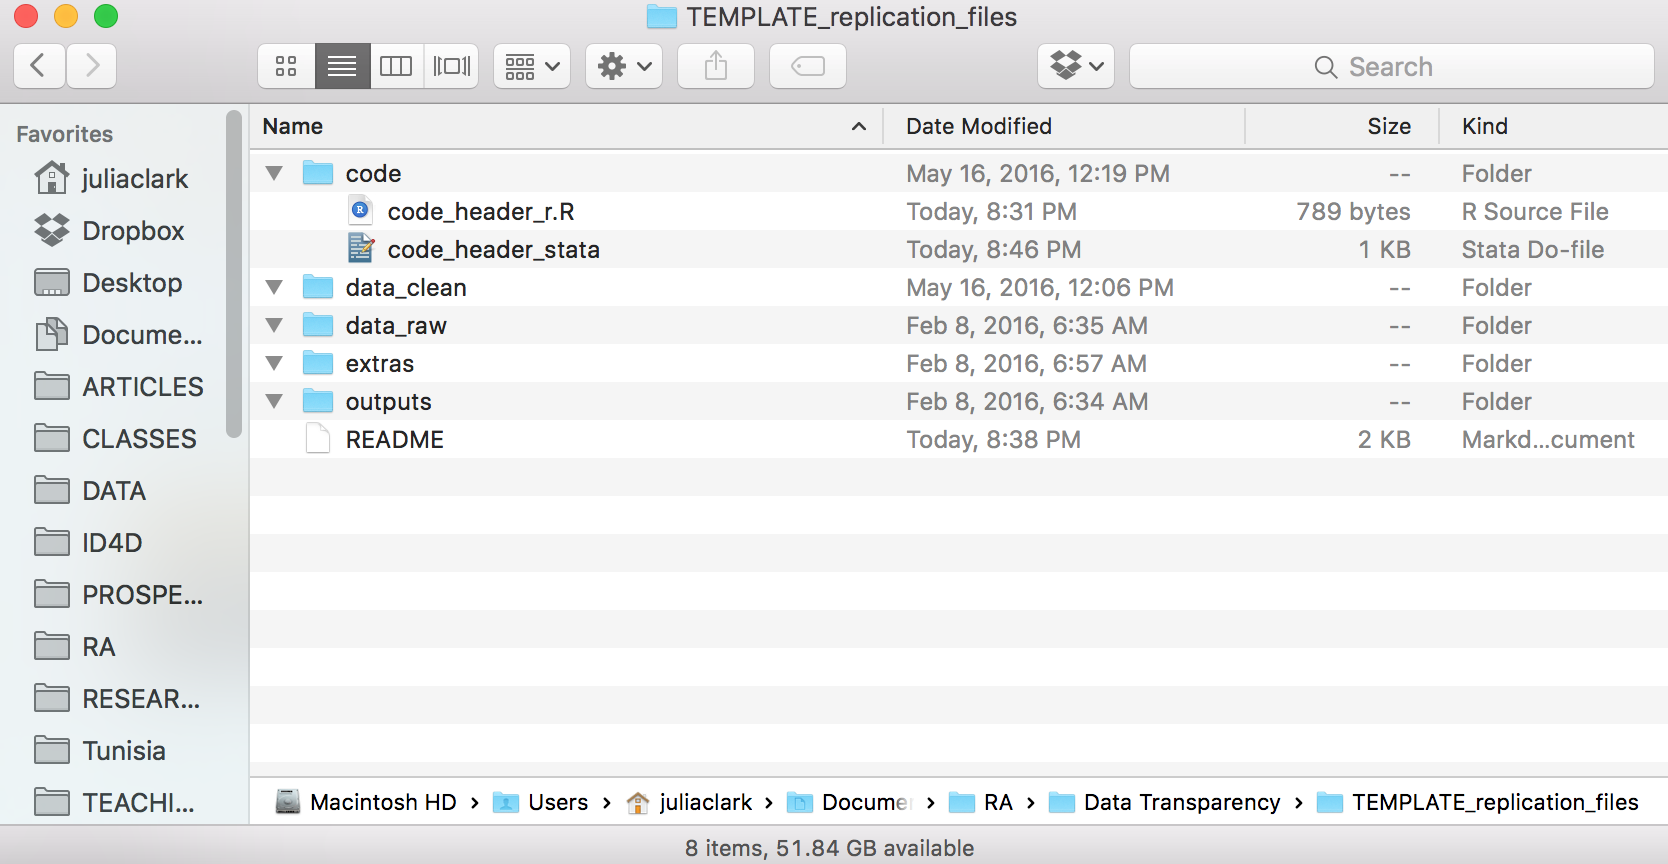
\includegraphics[width= \textwidth]{pdel_structure}
			\end{figure}
	\end{frame}
	
%%%%% LITERATE PROGRAMMING	
	
\subsection{4. Literate Programming}	

	\begin{frame}{About Literate Programming}
		\begin{itemize}
			\item \textbf{What:} Writing code that it's legible to \textit{humans}
			\item \textbf{Why:} So you and others can better replicate your work (and to help you avoid mistakes!)
		\end{itemize}
	\end{frame}
	
	\begin{frame}{(The Most) Basic Principles}
		\begin{itemize}
			\item Structure and name files intuitively
			\item Difficult to comment/annotate too much
			\item White-space (e.g., spaces, tabs, returns) is your friend
		\end{itemize}
	\end{frame}
	
	\begin{frame}{Structure and Name Files}
 		
 		\begin{itemize}
 			\item	 Create separate scripts for merging/cleaning and data analysis, with a master-script for running it all
 			\item Give code, data files, and output logical names where possible 
 			\begin{itemize}
 				\item e.g., Number folders/files sequentially in the order they should be run
 			\end{itemize}
 		\end{itemize}
 	\end{frame}
 
	 \begin{frame}{Streamline \& Annotate Code}
	 	
	 	\begin{itemize}
	 		\item Add headers (see PDEL template)
	 		\item Format scripts so they're easily readable---e.g., indent code, use ample line breaks and spaces, standardize comment syntax
	 		\item Add comments to improve reader understanding; remove unhelpful/embarrassing comments
			\item Clearly label code sections, main analyses, outputs 
			\item Give variables intuitive names like \texttt{edu\_percent} rather than \texttt{v76}
			\item Label variables and values in Stata
			\end{itemize}
	 \end{frame}
	 	 
	 \begin{frame}{Use working directories}  
			\textbf{R}: \texttt{setwd("$\sim$/Documents/replication\_files")} \\
		 	\textbf{Stata}: \texttt{capture cd "$\sim$/Documents/replication\_files"}
		 	
		 	\bigskip
		 	
			 \begin{itemize}
			 	\item Saves you time, since you (or someone replicating your study) only have to change the path once if the files move AND your code will be shorter
			 	\item Particularly helpful if co-authors alternate between Mac (``/") and Windows (``$\backslash$") file extensions
			 \end{itemize}
	 \end{frame}

	
%%%%% VERSION CONTROL	
	
\subsection{5. Version Control}

	\begin{frame}{About Version Control}
		\begin{itemize}
			\item \textbf{What:} A system for managing iterative versions of files (code, data, manuscripts) over time and across collabrators
			\item \textbf{Why:} Keep original files, protect work, collaborate efficiently, streamline workflow, etc., etc.
		\end{itemize}
	\end{frame}

	\begin{frame}
	\centering
		\ig[width=.6\textwidth]{phd101212s.png}
	\end{frame}
	
	\begin{frame}{Principles of Version Control}
		\begin{itemize}
			\item Vault original, raw data files---do not save over!
			\item Changes to files should be documented and reversible
			\item Keep ``master" versions of files in working order; create copies before experimenting
			\item Reconcile independent changes  by different users
		\end{itemize}
	\end{frame}

	\begin{frame}{Manual Solutions}
			\begin{itemize}
				\item Create dated versions of files (save-as) for each substantive change 
				\item With each modification, re-run ALL code to make sure nothing is broken---helps if you have a master file to run all scripts!
				\item Check-in with coauthors to ensure multiple people aren't working on the same files at the same time
				\item Keep a simple text file log to remind yourself of the location/content of major changes
			\end{itemize}	
				
	\end{frame}
	
	\begin{frame}{Or let version control software do this for you!}
		\centering 
		\ig[width=\textwidth]{github-logo}
	\end{frame}

%% GITHUB	

	\begin{frame}{Version control software > Git > GitHub}
	
		\begin{itemize}
			\item \textbf{Version control software:} helps manage versions and edits to files (e.g., Microsoft Word's ``track changes", or Google Doc's ``suggestion" feature)---\href{https://en.wikipedia.org/wiki/List_of_version_control_software}{many options!}
			\item \textbf{Git:} Open-source, ``distributed model" of version control developed by creator of Linux
			\item \textbf{GitHub:} Free, web-based service that hosts Git ``repositories" and offers a variety of features for collaboration
		\end{itemize}
	\end{frame}
	
%	\note{**Version control** software help manage versions and edits to files. If you've used Word's ``track changes" feature, or Google Doc's ``suggestion" feature, these are also version control tools. But they are not very powerful. In Word, comments and track changes become unwieldy very quickly. Once you accept a change, there is no way to roll-back to a previous version of the document.
%	
%		There is a better way! Software specifically design for version-controlling that lets you *collaboratively* view, accept, and roll back changes at any stage in a file's development, and works for text files as well as code. There are a many options, but we will use **Git**, developed by Linux creator Linus Torvalds. Git is an open-source, distributed model of version control. This means that each user works with repositories (files) locally on their own computer, and then changes to these files can shared with other users.
%		
%		With Git, sharing between users can work in a number of ways. The easiest is through **GitHub**, a free, web-based service that hosts Git repositories and offers a variety of features for collaboration. If you're starting out with Git, the easiest way is through GitHub.
%	}
	
	\begin{frame}{Common problems that GitHub helps solve}
	
		\begin{itemize}
			\item \textbf{Tracking changes in code/text files}---who, what, where, when, preserved forever
			\item \textbf{Selectively reverting changes}---better than \texttt{ctrl + Z}
			\item \textbf{Experimenting}---easier than ``my\_code\_v2\_new.R"
			\item \textbf{Collaborating}---sharing/vetting/reconciling changes
		\end{itemize}
	\end{frame}
	
%	\note{TRACKING CHANGES: Track changes in Word is OK, but gets messy quickly and doesn't work for code or LaTeX.
%	
%	REVERTING CHANGES: You make some edits and later decide to undo them. If the doc is still open, hit `undo' a bunch of times. BUT, what if you wanted to keep the 3rd, change you made, but undo the 1st and 2nd? The only option is to undo them all, and then try to re-execute the ones you want to keep. This is a waste of time and you may screw up. And you're completely out of luck if you already closed the file. 
%	
%	EXPERIMENTING: There's a part of your file that you like, and another part that you want to experiment with. You can ``save as" a new version to experiment on, naming it something like "mydraft\_New". In the course of working on the ``new" version, you make a number of changes, but decide that you like some parts of the old version better. How do you integrate these two documents? Word' ``combine versions" is clunky and doesn't help with non-Word files. Instead, your project directory is likely to be littered by a graveyard of obsolete documents (mydraft\_final\_110817) that keep just in case but will quickly loose track of and probably never revisit.
%	}
%	\note{COLLABORATING: You are collaborating on a project with a number of coauthors, all contributing to drafts of code and/or manuscripts. Maybe you have a Dropbox set up to sync versions with, but there's always the possibility that two people will be working on the same file at the same time, resulting in conflicting changes between files that are a pain to resolve. Although Dropbox helps with sharing, it doesn't address either of the problems described above, which are compounded with multiple authors.}
		
	\begin{frame}{How do I use GitHub?}
	
		\begin{itemize}
			\item \textbf{GitHub website}---necessary for collaboration, but limitations
			\item \textbf{GitHub Desktop}---free desktop client for Windows/Mac, more user friendly than website
			\item \textbf{Command line (shell)}---optimal for advanced users
		\end{itemize}
	\end{frame}

%	\note{While it's possible to use *only*  the GitHub website, this requires the desire/ability to work in your files directly through the online interface. If you have a constant internet connection and work only in text files, this may be do-able. 
%	
%	However, a much easier option is to download the free **GitHub Desktop** client for Windows and Mac (for Linux, you have to use the command line, which you can also use on Macs and PCs). This lets you work on files locally and then sync them with the remote repositories hosted online.
%	
%	Advanced users can also take full advantage of Git features by using the command line (there are limitations to what the Desktop client can do, and sometimes it is buggy.}

	\begin{frame}{How to think about Git: A Metaphor}
	
		\begin{columns}
			\begin{column}	{.5\textwidth}
				\centering
				\ig[width=.7\textwidth]{Big-brother-poster1.png}
			\end{column}
			\begin{column}{.5\textwidth}
				Tell \nb{Big Brother Git} to watch a set of files (a ``repository") and it tracks every change within them, line-by-line.
			\end{column}
		\end{columns}
	\end{frame}
	
%	\note{**A metaphor:** Git is Big Brother. You tell it to watch a set of files by ``adding" or ``creating" a repository and then it tracks their every change. It tells you that changes have been made, and lets you enter  (``commit")  those changes into the official record along with detailed comments about what those changes were. 
%	
%	If you're working in a type of file that Git can read---e.g. text files and most code files---it even shows you line by line what those changes were. If you don't like a particular change or ``commit" later on, you can undo (``revert") it. 
%	
%	When you open GitHub Desktop, the interface seems somewhat counterintuitive, in that it's showing you files, but you can't open or edit them from within an app, like it seems like you should be able to from a file manager. But that's not what it's doing. Think of it more as Big Brother's dashboard for changes in your document, and the whole thing makes a lot more sense.}
	
%	\begin{frame}{How to think about Git: An Analogy}
%		As described by \href{https://www.hastac.org/blogs/harrisonm/2013/10/12/github-academia-and-collaborative-writing}{Harrison Massey of hastac}, some Git processes are analogous to the \nb{analog editing process}.
%	\end{frame}
	
	\begin{frame}{What GitHub is NOT ... }
	
		\begin{enumerate}
			\item \textbf{Dropbox.} Git tracks changes in files and GitHub let's you sync/track/view/edit those changes online and with collaborators. Dropbox is a hard drive in the cloud. 
			\item \textbf{File Manager/GUI.} GitHub desktop may \textit{look} sort of like Finder (Mac) or Explorer (PC), but its function is not to let you find, click on, or open files; it's unit of operation is \textit{changes within those files}.
		\end{enumerate}
		
		
		\bigskip \centering
		\nb{Also, most useful for text files (.txt, \LaTeX, Markdown, Stata, R code, etc.); not useful for PDF, Word, Excel.}
	\end{frame}

	\begin{frame}{GitHub Prep}
		If you haven't already ...
		
		\begin{itemize}
			\item \textbf{Make sure you have a good text editor.} Notepad (PC) and TextEdit (Mac) will work (if you set TextEdit default file format to \texttt{.txt} and not \texttt{.rtf}). Or get a more powerful editor like \href{https://atom.io/}{Atom}. 
			\item \textbf{Create an account at \href{http://www.github.com}{GitHub}.} This gives free \textit{public} repositories, but go to the \href{https://education.github.com/}{education section} and click ``request a discount" to get free \textit{private} repositories. 
			\item \textbf{Download and install \href{https://desktop.github.com/}{GitHub Desktop}.} Then open and log in using your GitHub account.
		\end{itemize}
	\end{frame}

	\begin{frame}{Basic vocabulary}
	
		\begin{itemize}
			\item \nb{\textbf{Repository:}} A set of files (in a folder) that you have told Git to track, along with its associate .git files. A \nb{local} repository is the copy on your computer; a \nb{remote} repository is the copy synced online.
			\item \nb{\textbf{Commit:}} A labeled change or series of changes to files. Git tracks every change you make, and then you group these changes as desired into a ``commit" that can be commented on, reverted, etc.
		\end{itemize}
	\end{frame}

	\begin{frame}{1. Create a NEW repository}
	
	Within \textbf{GitHub Desktop}, click on ``$+$" and then ``create" to make a new repository with a name and location of your choice. This creates a new folder that will be empty except for some hidden files (e.g., a .git directory).
	
		\bigskip \centering
		\ig[width=.8\textwidth]{add_repository.png}
	\end{frame}
	
		% Now, you should see a the repository you've created on the left (although yours will have a computer icon next to it, since it's a \textit{local repository}, i.e., only on your computer and not yet synched to GitHub): ![](images/) 
		
	\begin{frame}{2. Add a text file to your repository}
		\begin{itemize}
			\item Create a new text file on your computer called ``README" as you normally would, and \textit{save it in your repository location}.
			\item  This should be a plain text file (.txt) or Markdown file (.md), not a rich text format file (.rtf). 
		\end{itemize}	
	\end{frame}
	
	\begin{frame}{3. Commit this change in GitHub Desktop}
		If you open up the desktop client, it will look something like this: 
		
		\bigskip
		\centering
		\ig[width=.8\textwidth]{add_readme.png}
	\end{frame}

	% Changes made to the repository—in this case, adding a file called "README"—are highlighted in blue. The right-hand pane is grey because there have been no changes inside the README file; the only change to the repository was adding it. Let's commit (i.e., officially record) this change by adding a short summary, optional description, and clicking Commit to master.

	\begin{frame}{4. Add text to README and commit changes}
		\textbf{Add some text to your file and save.} If you go back to the Desktop client, you will now see something like this: 
		
		\bigskip
		\centering
		\ig[width=.7\textwidth]{edit_readme.png}		
	\end{frame}
	
	\begin{frame}{5. Edit README text and commit changes}
		\textbf{Make and save changes to your text}, then go back to GitHub Desktop. In the right-hand pane, additions will appear in \textcolor{green}{green} and deletions will appear in \textcolor{red}{red}:
			\centering
			\ig[width=.7\textwidth]{edit_readme2.png}
		
		
		\bigskip
		Note that the unit of change is the \textit{paragraph}, so changing ``?" to ``!" involved deleting/adding the whole phrase.
	\end{frame}
 	% Commit your changes.

	\begin{frame}{6. Undo the last commit}
		If you're unhappy with your LAST commit (i.e., you disliked how it was grouped or labeled), you can \textbf{click the ``Undo"} button at the bottom of the list of uncommitted changes:
		
		\centering
		\ig[width=.5\textwidth]{undo.png}	
				
		Now, these changes will appear again in the "uncommitted changes" window for you to regroup or relabel.
	\end{frame}

	\begin{frame}{6. Revert a previous commit}
		If you're unhappy with the CHANGES in a commit themselves, you can undo them by \textbf{reverting} a commit. To do this, \textbf{switch to the ``History" tab} at the top of the window and view all your previous commits. Select the commit, navigate to the dropdown menu, and click \textbf{``Revert"}: 
		
		\bigskip
		\centering
		\ig[width=.8\textwidth]{revert.png}		
	\end{frame}
	
	% When you revert the commit and return to the text file on your computer, you'll see that the last change has been undone, and the revert has now been recorded as a new commit (so you can revert your revert if you change your mind again).

	\begin{frame}{7. Publish repository to your online account}
		So far, we've been working in a \textbf{local repository}--one that that you created on your computer. 
		
		\bigskip
		This may be useful to you, but to collaborate on projects you'll need to publish the repository to the web (i.e., make a \textbf{remote repository}). $\rightarrow$  \nb{Do this by \textbf{clicking ``publish''}:}
		
			\bigskip
			\centering
			\ig[width=.2\textwidth]{publish.png}	
		
	\end{frame}

	\begin{frame}{8. View your repository \& changes online}
		When you login to GitHub online, you'll see the new repository and file you've added.
			\centering
			\ig[width=.8\textwidth]{git_online.png}
	\end{frame}
	
	\begin{frame}{9. Edit the file online \& sync with local repository}
		Click on the README file and then click the edit button (the pen). \nb{(A)} \textbf{Make some changes and then commit}. Then go back to the Desktop client and \textbf{click ``Sync"}. \nb{(B)} Your new commit will appear in the \textbf{history tab}.
		
		\bigskip
		\begin{columns}
			\begin{column}	{.5\textwidth}
				\centering
				\nb{(A)}
				\ig[width=\textwidth]{online_edit.png}
			\end{column}
			
			\begin{column}{.5\textwidth}
				\centering
				\nb{(B)}
				\ig[width=\textwidth]{sync.png}
			\end{column}
		\end{columns}

	\end{frame}
	
	\begin{frame}{What's next?}
		That was very very basic. To really use Git, explore these great features with weird names ... 
		
		
		\small
		\begin{itemize}
			\item \textbf{\nb{Cloning} online repositories}---copies an online repository onto your local hardrive so you can work offline
			\item \textbf{\nb{Forking} online repositories}---duplicates \textit{someone else's} shared repository and lets you use/change/build on it without affecting their original work
			\item \textbf{\nb{Branching} a repository}---lets you (and collaborators) experiment with changes that can be merged into the ``master" version of the files
			\item \textbf{Initiating a \nb{pull request}}---submits your commits to be merged into a forked/branched repository (accepted/rejected by collaborators)
		\end{itemize}
	\end{frame}

	\begin{frame}{Git Resources}
	Too many to name, but some good places to start:
	\begin{itemize}
		\item \href{http://www.chronicle.com/blogs/profhacker/a-gentle-introduction-to-version-control/23064}{Gentle intro to version control}
		\item \href{https://www.hastac.org/blogs/harrisonm/2013/10/12/github-academia-and-collaborative-writing}{GitHub and collaborative writing in academia}
		\item \href{http://www.chronicle.com/blogs/profhacker/forks-and-pull-requests-in-github/47753}{Forks and pull requests}
		\item \href{http://blog.scottlowe.org/2015/01/14/non-programmer-git-intro/}{Non-programmer's intro to Git using command line}
		\item \href{http://blog.scottlowe.org/2015/01/27/using-fork-branch-git-workflow/}{Fork-branch workflow using command line (but useful to read for Desktop as well)}
	\end{itemize}
	\end{frame}

%%%%% DYNAMIC DOCS	

	\begin{frame}{[Dynamic Docs]}
	You can take reproducible research a step further by integrating code \textit{into your manuscript}. No need to copy-and-paste results from statistical software (annoying and error-prone); just click the button and everything reproduces. 
	
	
	\begin{itemize}
		\item \href{http://rmarkdown.rstudio.com/}{RMarkdown}
		\item \href{http://www.haghish.com/statistics/stata-blog/reproducible-research/markdoc.php}{Stata Markdoc} or \href{http://repec.sowi.unibe.ch/stata/texdoc/}{Stata texdoc}
	\end{itemize}
		
	\end{frame}

%%%%%%%%%%%%%%%  	PHASE 3: DISSEMINATION %%%%%%%%%%%
\section{Phase III: Dissemination}

	\begin{frame}{Steps}
	  	\centering
	  	\ig[width=\textwidth]{iii_dissemination}
	\end{frame}
	
%%%%% PREP FOR REPLICATION	
	
\subsection{6. Prepare for Replication}

	\begin{frame}{Why do we care if our code is reproducible?}
		\begin{itemize}
			\item \textbf{Unselfish reasons}---part of the scientific process and a public good
			\item \textbf{Selfish reasons}---make code more usable for yourself, catch potentially embarrassing errors before they become public, boost your transparency credibility
		\end{itemize}
		
	\end{frame}

	\begin{frame}{Replication files should ...}
	
		\begin{itemize}
			\item Be complete but parsimonious
			\item Run and reproduce results with one click
			\item Be readable and interpretable by humans
			\item Protect personal information
		\end{itemize}
		
		\bigskip
		
		\textbf{Caveat: }There is no single, perfect way to organize or prepare files for replication. Do what works for you (as long as it meets the above criteria)!
	\end{frame}

	\begin{frame}{5 Steps for Prepping Files}
			\begin{enumerate}
				\item Set-up
				\item Initial replication
				\item De-identify
				\item Edit
				\item Final replication
			\end{enumerate}
	\end{frame}
	  
		 \begin{frame}{1. Set Up}
		 	Create a \textit{new}, clearly organized folder structure for replication that you add to selectively.
		 	
		 	\begin{itemize}
		 		\item \textbf{Purpose:} 
		 		\begin{itemize}
		 			\item Ensure files are \textcolor{burntorange}{complete/parsimonious, legible}
		 			\item Protect original files
		 		\end{itemize}
		 	\end{itemize}
		 	
		 \end{frame}
		  
		 \begin{frame}{Create}
		 	\begin{enumerate}
		 		\item \textbf{A new, empty replication folder} \textit{within} your project directory (e.g., ``\texttt{replication\_files}") 
		 		\item \textbf{Subfolders:} \textit{Same as File Management tips!}
		 			\begin{itemize}
		 				\item \texttt{/code} --- scripts
		 				\item \texttt{/data\_clean} --- manipulated data
		 				\item \texttt{/data\_raw} --- original data
		 				\item \texttt{/output} --- generated tables, graphs, etc.
		 				\item \texttt{/extra} --- misc. extras (e.g., code book)
		 			\end{itemize}
		 			\item \textbf{A ``README.txt" file} to document contents, sources, software/system versions, other info necessary for replication/comprehension.
		 	\end{enumerate}
		 \end{frame}
		
		 \begin{frame}{2. Initial Replication}
		 	\textit{Copy} (don't move!) over data and code files into the replication folder and try to replicate your results.
		 	
		 	\bigskip
		 	
		 	\textbf{Purpose:}
			 	\begin{itemize}
			 		\item Make sure your code actually runs and \textcolor{burntorange}{reproduces} before you tinker with structure and formatting
			 		\item Build up your replication folder with \textcolor{burntorange}{complete and parsimonious} data/code files
			 	\end{itemize}
		 \end{frame}
		 
		\begin{frame}{Check Analysis}
			Easier to start with final analysis and work backwards to data cleaning/merging. 
			
			
			\begin{enumerate}
				\item Copy original analysis script(s) into \texttt{replication\_files/code}
				\item Copy cleaned dataset(s) used for analysis into \texttt{replication\_files/data\_clean}
				\item Run code without changes (except for wd)
				\item Fix any bugs in the code, address discrepancies with previous results
			\end{enumerate}
		\end{frame}
		
		\begin{frame}{Check Data Clean/Merge}
			\begin{enumerate}
				\item If separate from analysis, copy original merge/cleaning script(s) into \texttt{replication\_files/code}
				\item Copy original dataset(s) to \texttt{replication\_files/data}
				\item Run merge/clean code without changes (except for wd)
				\item Rerun the analysis code from above on the newly cleaned/merged data file
				\item If you get different results than step \#1, there is a discrepancy with  merging/cleaning code---fix it!
			\end{enumerate}
		\end{frame}
		
	\begin{frame}{3. De-Identifying Individual-Level Data}
		Now you know the code works and replicates, congratulations! The next step is to ensure that any shared files \textit{do not contain} data that could be used to identify individuals. 
		
		\bigskip
		
		\textbf{Purpose:} 
		\begin{itemize}
			\item Ensure you are \textcolor{burntorange}{protecting individuals' identity and private information}---this is an ethical issue for researchers, and a potential safety issue for participants
			\item Comply with legal, research board or funder requirements (e.g., HIPAA and IRB in the US) 
		\end{itemize}
		
	\end{frame}

	\begin{frame}{What does ``de-identifying" mean?}
		\textbf{Two types of identifiers:}
		
		\begin{enumerate}
			\item \textcolor{burntorange}{Direct:} Variables that is explicitly linked to the subject---\textit{e.g., name, email, address, ID number, phone number, etc.}
			\item \textcolor{burntorange}{Indirect:} Variables that, in combination, could be used to identify individuals---\textit{e.g., gender, dates (birth, program admission, etc.), geographic location (village, GPS), unusual occupations or education, etc.}
		\end{enumerate}
		
		\bigskip
		
		See \href{https://fpf.org/wp-content/uploads/2016/04/FPF_Visual-Guide-to-Practical-Data-DeID.pdf}{this useful infographic}.
	\end{frame}

	\begin{frame}{Example of Indirect Identifiers}	
		\begin{itemize}
			\item You survey teachers and collect information on \textit{gender}, \textit{classes taught}, and \textit{age}.
			\item If there is only one \textit{female}, \textit{third-grade} teacher \textit{aged 40-49} at a particular school, she is not anonymous in your data
		\end{itemize}
	\end{frame}		

	\begin{frame}{Dealing with Direct Identifiers}
		In general, direct identifiers---e.g., name, address, mobile number, ID number---should \textit{never} be made public. 
		
		\bigskip
			
		\textbf{Options:}
		\begin{itemize}
			\item Remove variables from shared dataset
			\item Pseudonymize data: replace identifiers with ``pseudonyms" that may be reversible or non-reversible---e.g., give people random names or ID numbers---goal is to be able to link datasets
		\end{itemize}
	\end{frame}	
	
	\begin{frame}{Solutions for Direct Identifiers}
		 \centering 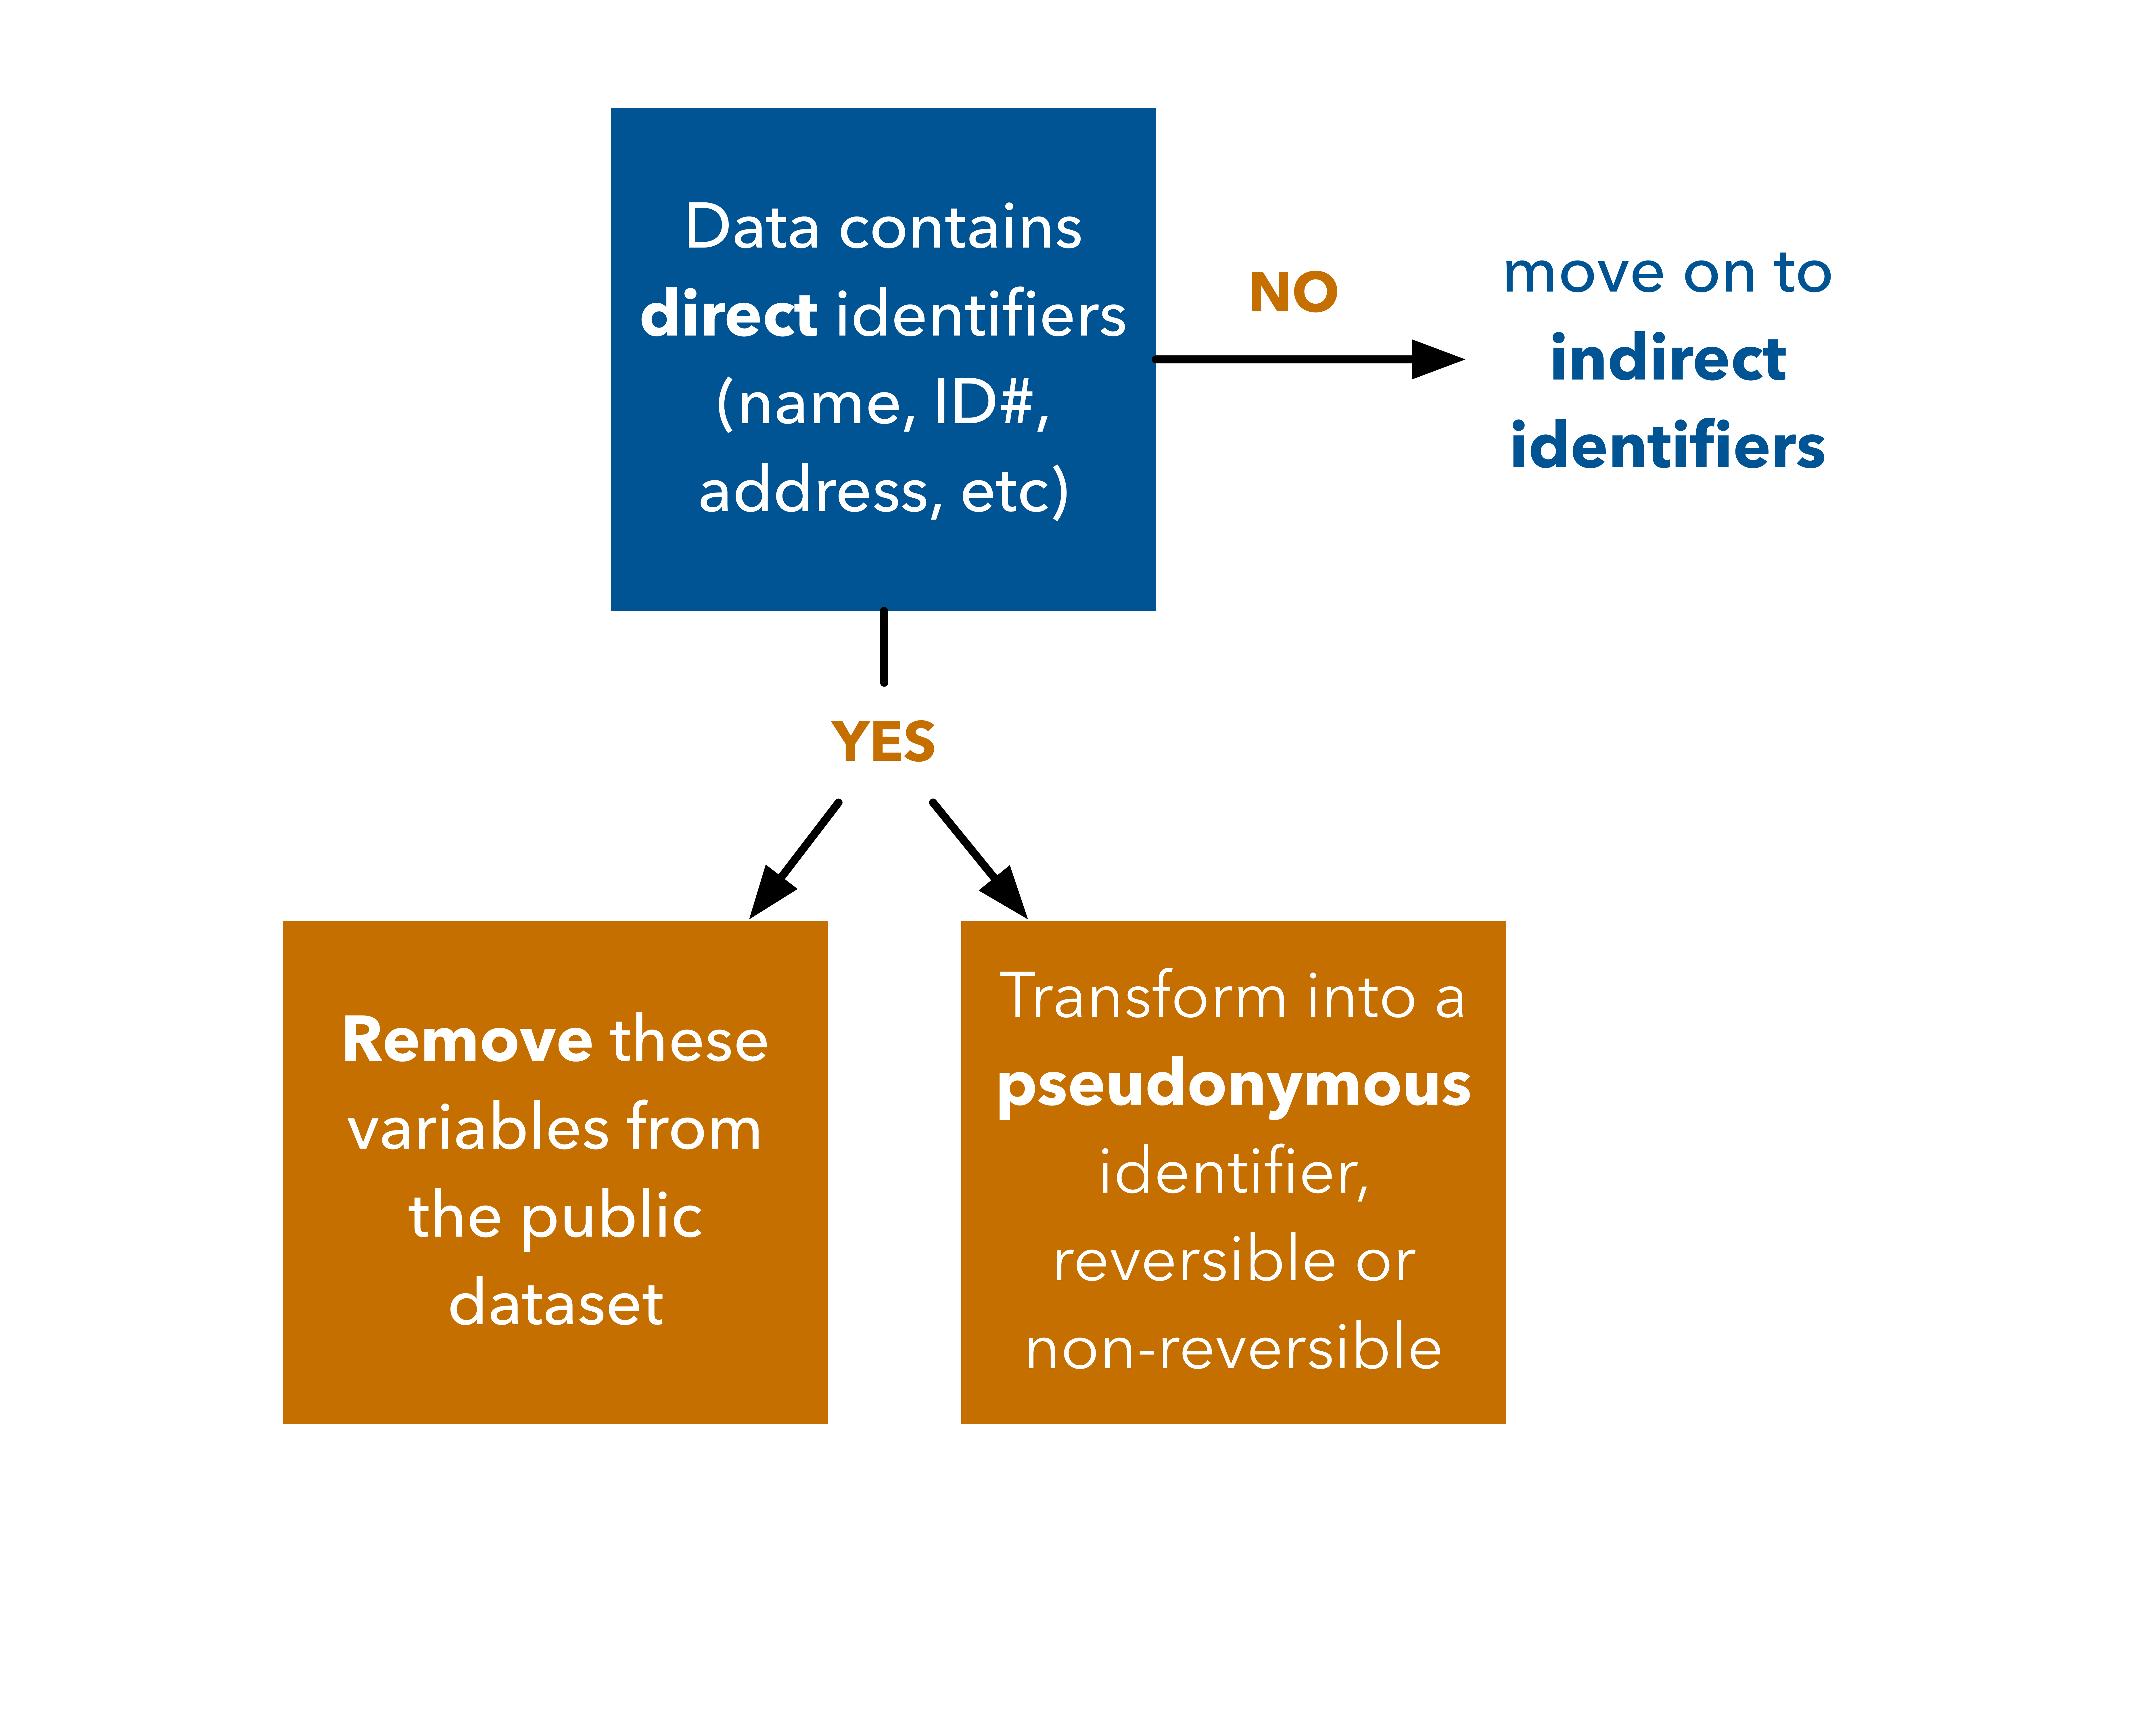
\includegraphics[width=.9\textwidth]{de-identification_direct.png}
	\end{frame}
	
	\begin{frame}{What is Sufficient De-Identification for Indirect Identifiers?}
	
		\begin{enumerate}
			\item \textbf{Determine Risk} = Pr(de-identifying) $\times$ sensitivity of data
			\item \textbf{Set k-anonymous level:} each record cannot be distinguished from at least $k-1$ other individuals who also appear in the data set
			\item \textbf{Select appropriate method(s) of de-identification:} aggregating data, removing certain variables or observations, reducing information/detail, adding random noise or values 
		\end{enumerate}
	\end{frame}
	
	\begin{frame}{The Problem}
		 \centering 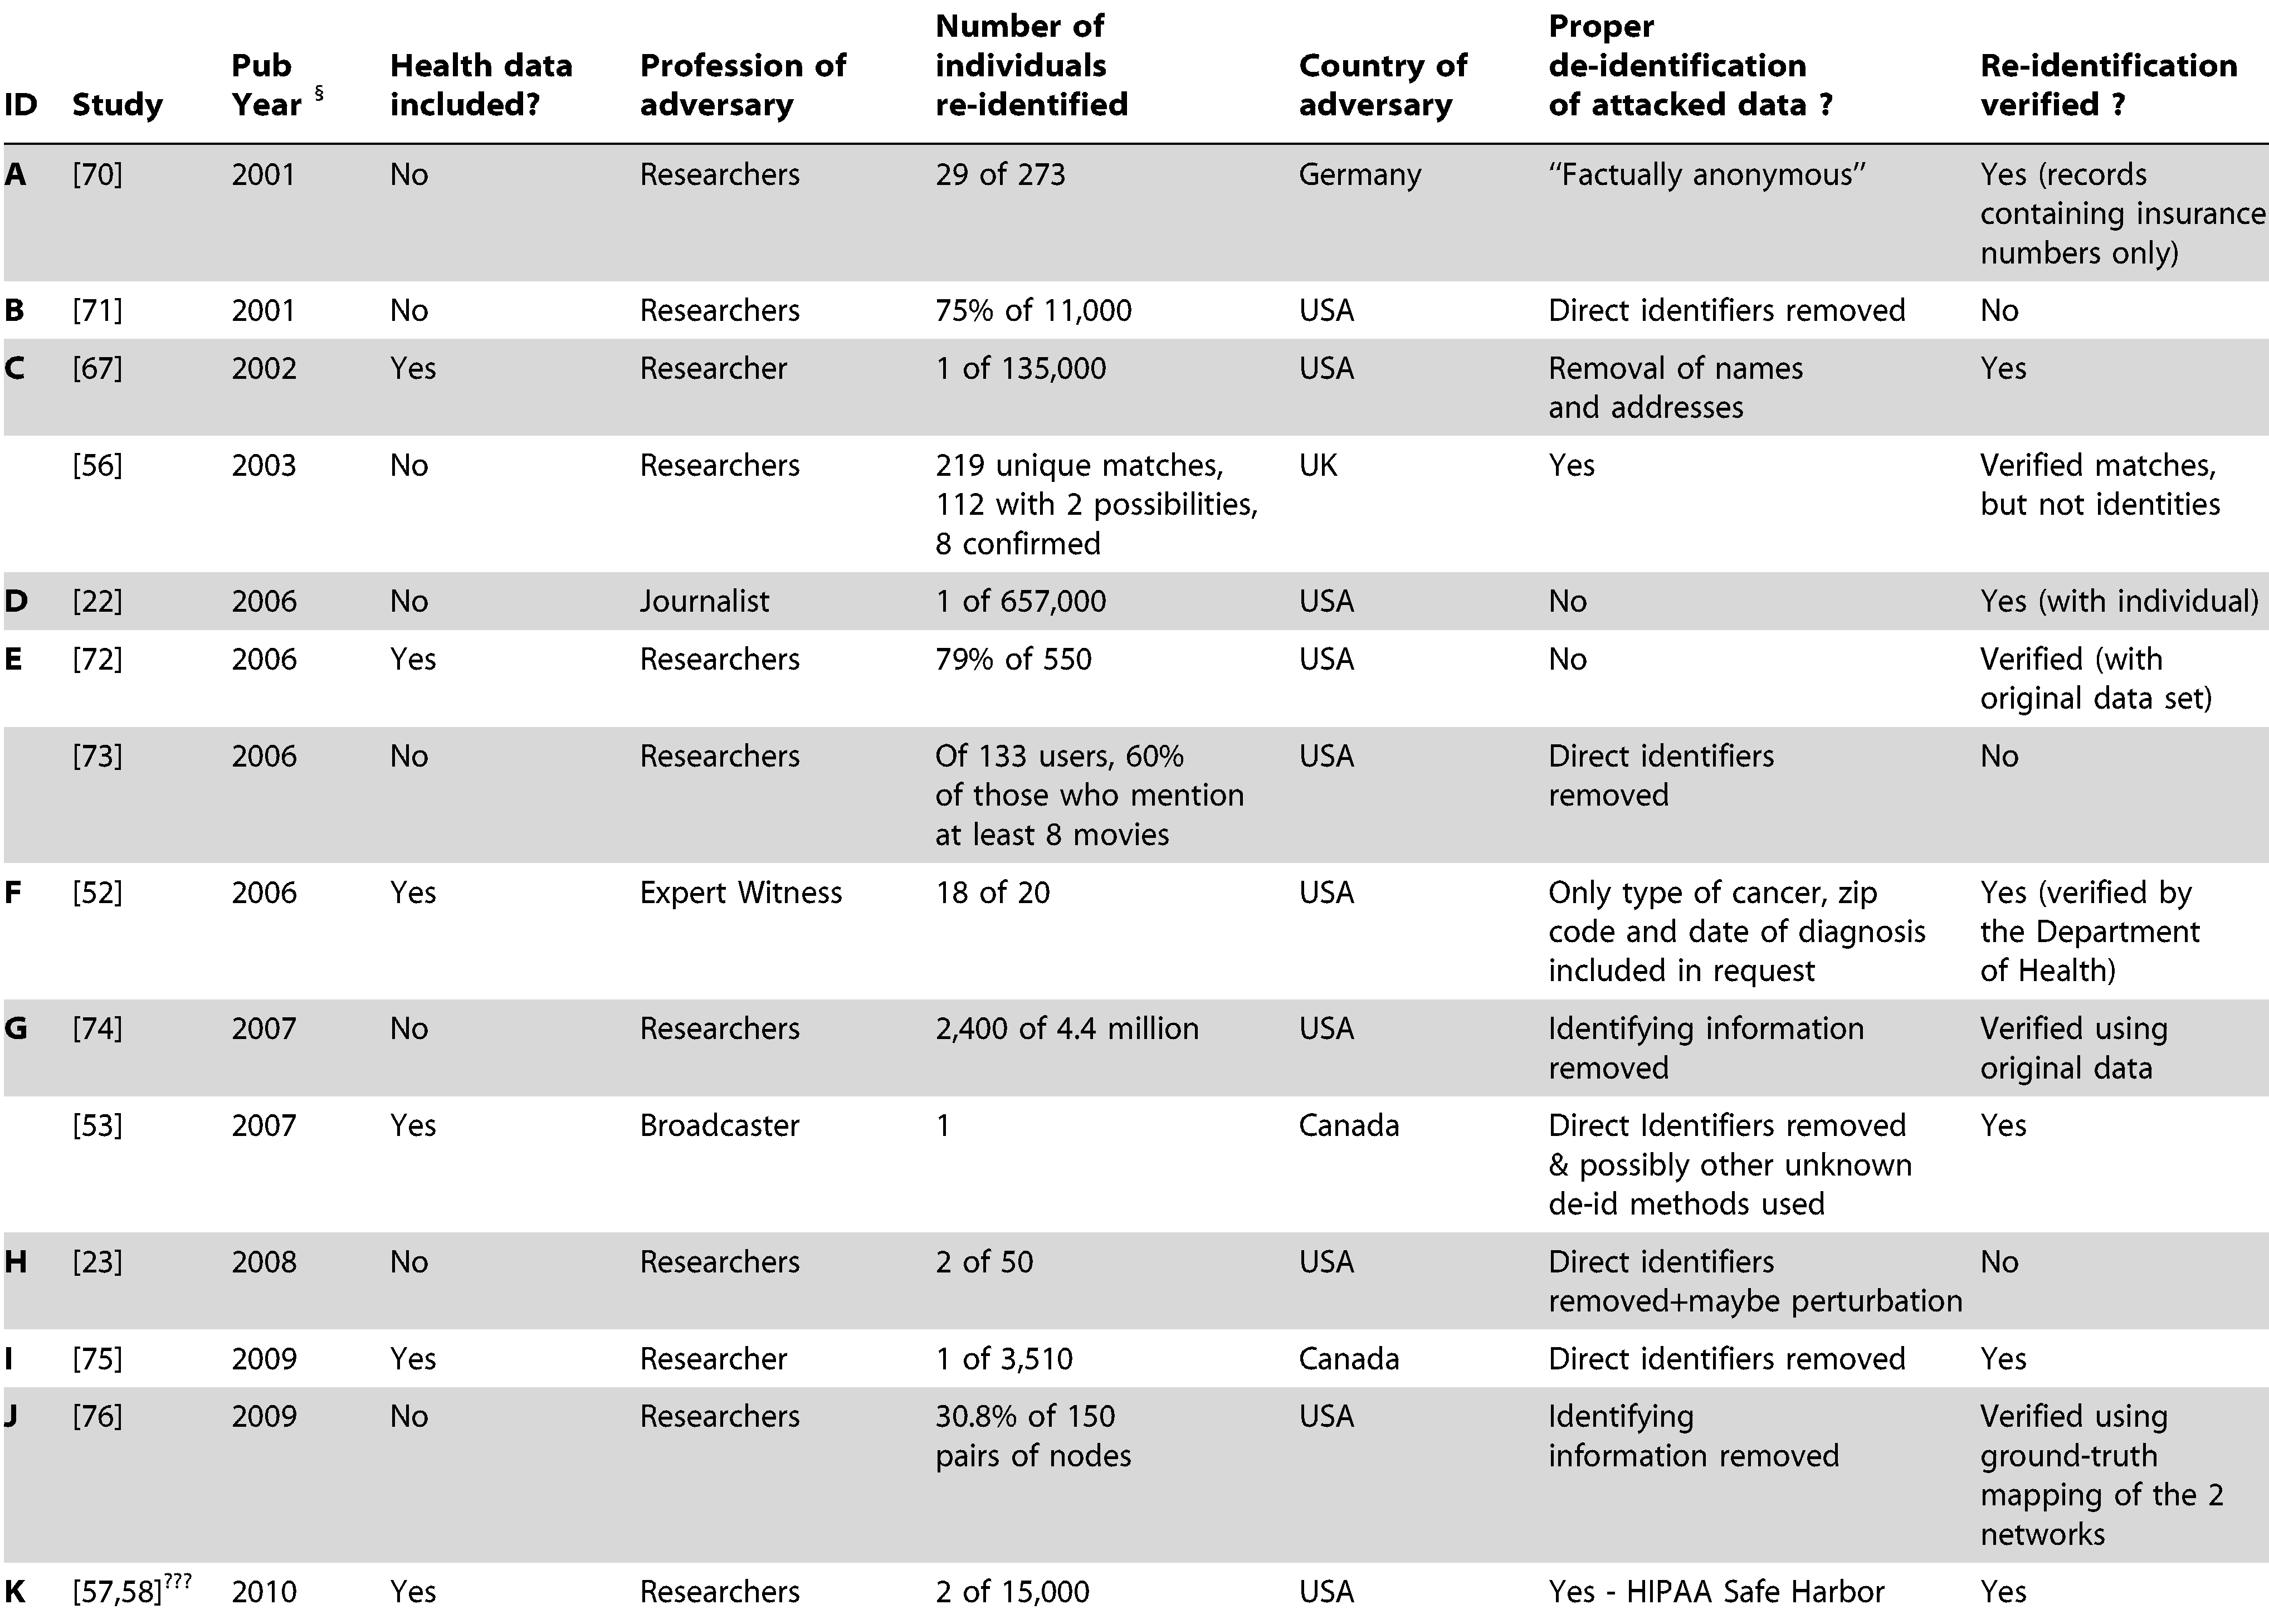
\includegraphics[width=.85\textwidth]{reidentification.png}
		 
		 \tiny{Source: El Emam et al. 2015. ``A Systematic Review of Re-Identification Attacks on Health Data." PLOS One. }
	\end{frame}
	
	\begin{frame}{Example of K-anon where k=3}
			 \centering 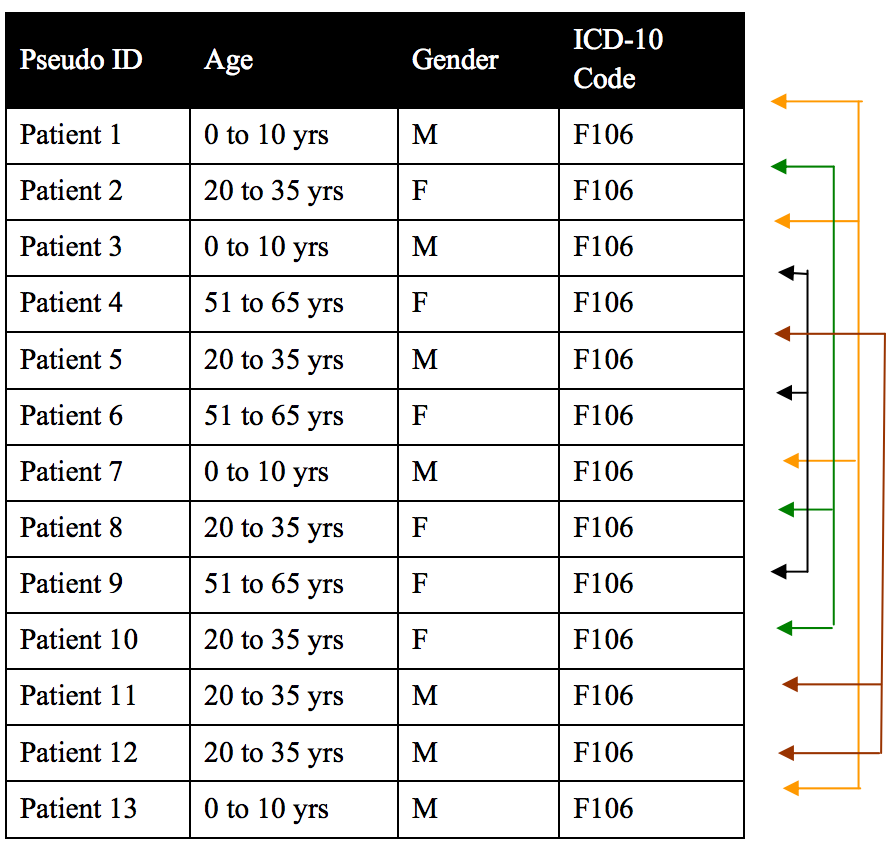
\includegraphics[width=.6\textwidth]{images/k-3.png}
	\end{frame}
	
	\begin{frame}{Solutions for Indirect Identifiers}
		\centering \includegraphics[width=1.1\textwidth]{images/de-identification_indirect.png}
	\end{frame}
	
	\begin{frame}{Trade-off: \textcolor{burntorange}{Usefulness} $\Longleftrightarrow$ \textcolor{burntorange}{Anonymity}}
		
		\begin{itemize}
			\item \textbf{Aggregating}---lose ability to replicate any individual-level analysis
			\item \textbf{Removing variables}---may not be able to replicate specific models
			\item \textbf{Reducing information}---adds noise to models
			\item \textbf{Remove observations}---adds bias if non-random
			\item \textbf{Adding random noise/values}---adds noise, obviously
		\end{itemize}	
	
	
	\bigskip
			See \href{http://www.ehealthinformation.ca/wp-content/uploads/2014/08/2010-Risk-based-de-identification-of-health-data.pdf}{here} and \href{http://www.ehealthinformation.ca/wp-content/uploads/2014/08/2009-Tools-for-De-Identification-of-Personal-Health.pdf}{here} for more discussion of appropriate thresholds, methods, and tools for de-identification.

	\end{frame}
	
	\begin{frame}{Good Practices}
			\begin{itemize}
				\item Include code for de-identified data for transparency (as long as the code itself doesn't compromise anonymity) 
					\begin{itemize}
						\item e.g., censor code that sets the seed for a random draw to generate new ID numbers and could be used to re-identify individuals
					\end{itemize}
				\item If identifiers \textit{aren't} used for analysis, de-identify early in merging/cleaning process
				\item Store original data with PII securely---if you're using Dropbox, see \href{https://github.com/PolicyDesignEvaluationLab/Transparency-Initiative/wiki/Tips:-Protocol-for-Sharing-Data-via-Dropbox}{PDEL GitHub wiki} for tips on sharing with RAs in a way that protects PII data
			\end{itemize} 	
	\end{frame}
		
 	\begin{frame}{4. Edit and Organize Files for Clarity}
 	Now we have working files that are de-identified; the next step is to clean and annotate them to improve usability. 
 	
 	
 	\bigskip
 	
 		\textbf{Purpose:}
 		\begin{itemize}
 			\item Ensure files are \textcolor{burntorange}{legible} in terms of structure and content
 		\end{itemize}
 	\end{frame}
  
 	\begin{frame}{Basic steps}
 		\begin{itemize}
 			\item Structure and name files*
 			\item Streamline and annotate code*
 			\item Document file and folder contents
 		\end{itemize}
 		
 		
 		\bigskip
 		\nb{*Already done if you follow the literate programming tips in Phase II!}
 	\end{frame}
 
\begin{frame}{Document File and Folder Content}
	\begin{itemize}
		\item Update the README file to describe contents of replication folders
		\item If necessary, include codebook in ``\texttt{/extra}" folder
		\item Track and document packages, software versions
		\begin{itemize}
			\item \textbf{R:} \texttt{sessionInfo()}
			\item \textbf{Stata:} \texttt{version}
		\end{itemize}
	\end{itemize}
\end{frame}
	

\begin{frame}{5. Final Replication}
	
		Now that you have cleaned/reorganized script files \dots 
		
		
		\begin{itemize}
			\item Shutdown or clear your Stata/R memory
			\item Rerun the entire process---including data merging, cleaning and analysis---to make sure the editing process didn't break anything
			\item Testing on a friend (or RA's) computer can also be a final check
			\item Once discrepancies are addressed, the files are ready for sharing!
		\end{itemize}
	
\end{frame}

%%%%% SHARE DATA AND CODE	
		
\subsection{7. Share Data and Code}

	\begin{frame}{About Sharing Data and Code}
		\begin{itemize}
			\item \textbf{What:} add study materials to an online repository
			\item \textbf{Why:} lasts longer than personal website, more searchable, future proof
			\item \textbf{Concerns:} 
				\begin{itemize}
					\item Can usually be embargoed, or you can provide only what is necessary for replication (e.g., leave out other survey Qs)
					\item Biggest risk isn't having your data/ideas stolen, it's having your research ignored! (King 1995)
					\item Difficult if proprietary
				\end{itemize}
		\end{itemize}
	\end{frame}
	
	\begin{frame}{Where to Share}
		Depends on discipline, find appropriate registry at \url{http://www.re3data.org/}. Or check out ... 
		
		\begin{itemize}
			\item \textbf{\href{https://dataverse.harvard.edu/}{Harvard’s Dataverse} }
			\item \href{https://osf.io/}{Open Science Framework}
			\item \href{https://www.openicpsr.org/openicpsr/}{OpenICPSR}
			\item \href{https://figshare.com/}{figshare}
			\item \href{http://datadryad.org/}{Data Dryad}
			\item University library (e.g., \url{http://library.ucsd.edu/dc/rdcp/collections})
		\end{itemize}		
	\end{frame}

%%%%% META-ANALYSIS	

\subsection{8. Meta-Analysis}
	
	\begin{frame}{About Meta-Analysis}
		\begin{itemize}
			\item \textbf{What:} Statistical analysis of a group of studies to derive a pooled estimate of the effect of a treatment; may be part of a ``systematic review"
			\item \textbf{Why:} Because individual study estimate may be biased or contain random error
		\end{itemize}
	\end{frame}

	\begin{frame}{One Study = One Data Point}
		That experiment you just ran with 3,685 participants? It's one data point among many other studies.
		\centering
		\textit{Even with the same data}, results may vary ... 
		
		
		\bigskip
		\ig[width= \textwidth]{truth-vigilantes-soccer-calls2}
	\end{frame}
	
	\begin{frame}{Who Does Meta-Analysis?}
		\begin{itemize}
			\item \href{https://www.campbellcollaboration.org/}{Campbell Collaboration} (policy)
			\item \href{http://www.3ieimpact.org/}{3ie} (development)
			\item Cochrane Collaboration (medicine)
			\item What Works Clearinghouse (US Gov’t, Education) 
			\item CLEAR (US Gov’t, Labor)
			\item MAER-NET (Economics)
			\item You!
		\end{itemize}
	\end{frame}
	
	\begin{frame}{Basic Steps}
	Using a PAP or ``protocol" (and assuming NO publication bias!) ...
	
	
		\begin{enumerate}
			\item Determine which studies to include 
			\item Determine which outcomes to measure (e.g., discrete, continuous)
			\item Select model for ``meta-regression" (e.g., RE, FE, etc.)
		\end{enumerate}
	\end{frame}
	
	\begin{frame}{Funnel Plots}
		Scatter plot of study effect sizes vs. study prevision (e.g., SE of study treatment effect)
		
		
		\bigskip \centering
		\ig[width=.8\textwidth]{funnel.png}	
		
		\small \textit{Source: BMJ 2011}
	\end{frame}
	
%%%%%%%%%%%%%% ETC. %%%%%%%%%%%%%%%%%
\section{Etc.}

\begin{frame}{Solutions at the Institutional/Discipline Level}
	\begin{itemize}
		\item \textbf{Design-based publication:} AKA ``registered reports," moves peer review before data analysis (\href{https://osf.io/8mpji/wiki/home/}{example})
		\item \textbf{Incentives for transparency, replication, meta-analysis:} See BITSS \href{http://www.bitss.org/lr-prizes/}{prizes} and \href{http://www.bitss.org/ssmart-grants/}{awards}, \href{https://osf.io/prereg/}{OSF pre-registration challenge}, etc.
		\item \textbf{Change norms:} e.g., journal/disciplinary standards for data sharing
		\item \textbf{Training:} Like this! more at BITSS, \href{https://cos.io/our-services/training-services/}{Center for Open Science}, etc.  
		\item \textbf{Tenure:} ``Adherence to the replication standard should be part of [tenure] judgment" (King 1995)
	\end{itemize}
\end{frame}

\begin{frame}{Selected Reading}
\footnotesize
\begin{itemize}
	\item \textbf{Transparency:} \href{https://github.com/garretchristensen/BestPracticesManual}{BITSS Best Practices Manual}
	\item \textbf{Replication:}  \href{http://www.jstor.org/stable/1806061?seq=1\#fndtn-page\_scan\_tab\_contents}{Dewald et al. (1986)}, \href{http://gking.harvard.edu/files/replication.pdf}{King (1995)}, \href{http://www.pnas.org/content/109/42/17028.long}{Fang et al. (2012)}, \href{https://fivethirtyeight.com/features/science-isnt-broken/}{FiveThirtyEight (2015)}, \href{https://www.cgdev.org/sites/default/files/CGD-Working-Paper-399-Clemens-Meaning-Failed-Replications.pdf}{Clemens (2015)}
	\item \textbf{Publication bias:} \href{http://www.nejm.org/doi/full/10.1056/nejmsa065779}{Turner et al. (2008)}, \href{http://journals.sagepub.com/doi/pdf/10.1177/0049124108318973}{Gerber \& Malhotra (2008)} \href{http://journals.plos.org/plosone/article?id=10.1371/journal.pone.0010068}{Fanelli (2010)}, \href{https://link.springer.com/article/10.1007/s11192-011-0494-7}{Fanelli (2011)}, \href{http://science.sciencemag.org/content/345/6203/1502}{Franco et al. (2014)}
	\item \textbf{P-hacking, fishing, researcher degrees of freedom, fraud:} \href{https://papers.ssrn.com/sol3/papers.cfm?abstract_id=1850704}{Simons, Nelson, Simonsohn (2011)}, \href{http://www.stat.columbia.edu/~gelman/research/unpublished/p_hacking.pdf}{Gelmen \& Loken (2013)}, \href{https://www.aeaweb.org/articles?id=10.1257/app.20150044}{Brodeur et al. (2016)}, \href{https://www.cmu.edu/dietrich/sds/docs/loewenstein/MeasPrevalQuestTruthTelling.pdf}{John et al. (2012)}
	\item \textbf{PAPs:} \href{https://www.aeaweb.org/articles?id=10.1257/jep.29.3.61}{Olken 2013}, \href{https://www.aeaweb.org/articles?id=10.1257/jep.29.3.81}{Coffman \& Niederle (2015)}, \href{http://onlinelibrary.wiley.com/doi/10.1111/0019-8676.00199/full}{Neumark 2001}
	% \item \textbf{Ethics in experiments:} \href{http://desposato.org/ethicsfieldexperiments.pdf}{Desposato (2014)}
	\item \textbf{De-identifying data:} \href{http://www.ehealthinformation.ca/wp-content/uploads/2014/08/2009-Tools-for-De-Identification-of-Personal-Health.pdf}{Tools for De-Identification}, \href{http://www.ehealthinformation.ca/wp-content/uploads/2014/08/2010-Risk-based-de-identification-of-health-data.pdf}{El Emam (2010)}
	\item \textbf{Literate programming:} \href{https://www.amazon.com/Workflow-Data-Analysis-Using-Stata/dp/1597180475}{Long (2008)}, \href{https://www.amazon.com/Reproducible-Research-Studio-Chapman-Hall/dp/1466572841}{Gandrud (2013)}, \href{http://www.brown.edu/Research/Shapiro/pdfs/CodeAndData.pdf}{Gentzkow \& Shapiro (2014)}
	\item \textbf{Meta-analysis:} \href{http://www.jstor.org/stable/2117925?seq=1\#page\_scan\_tab\_contents}{Card \& Krueger (1995)}, \href{https://www.amazon.com/Meta-Regression-Analysis-Economics-Business-Routledge/dp/0415670780}{Stanlet \& Doucouliagos (2012)}, \href{http://www.bmj.com/content/343/bmj.d4002}{BMJ (2011)}
	\end{itemize}

\end{frame}




\end{document}